% Created 2023-10-23 Mon 22:52
% Intended LaTeX compiler: pdflatex
\documentclass[presentation,smaller]{beamer}
\usepackage[utf8]{inputenc}
\usepackage[T1]{fontenc}
\usepackage{graphicx}
\usepackage{longtable}
\usepackage{wrapfig}
\usepackage{rotating}
\usepackage[normalem]{ulem}
\usepackage{amsmath}
\usepackage{amssymb}
\usepackage{capt-of}
\usepackage{hyperref}
\usetheme{MIS}
\author{vopuu}
\date{\today}
\title{}
\begin{document}


\section*{Transitioning from ML to DL}
\label{sec:org0509f3b}
\begin{frame}[label={sec:org069d3a7}]{Why Deep Learning?}
\begin{columns}
\begin{column}{0.6\columnwidth}
\begin{itemize}
\item \alert{\alert{Complexity}}: DL excels with complex data (images).
\item \alert{\alert{Data Size}}: Takes advantage of big data (Uniprot \(\gt 10^8\) sequences).
\item \alert{\alert{Automatic Features}}: No manual feature crafting needed.
\item \alert{\alert{Superiority}}: Outperforms ML in image and text generation.
\item \alert{\alert{End-to-End}}: Direct input-output, e.g., AlphaFold for protein folding.
\end{itemize}
\end{column}

\begin{column}{0.4\columnwidth}
\begin{center}
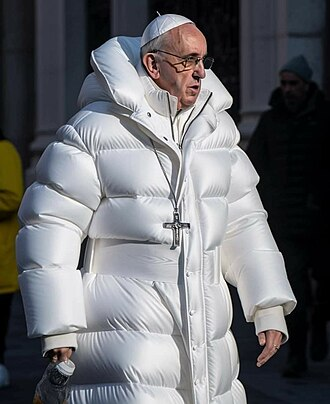
\includegraphics[width=.9\linewidth]{./img/midjourney.jpg}
\end{center}
(generated with midjourney)
\end{column}
\end{columns}
\end{frame}

\begin{frame}[label={sec:org7edfec0}]{Application of DL in biology}
\begin{center}
\Large AlphaFold, AI to predict the fold of globular proteins at the experimental accuracy
\end{center}

\begin{center}
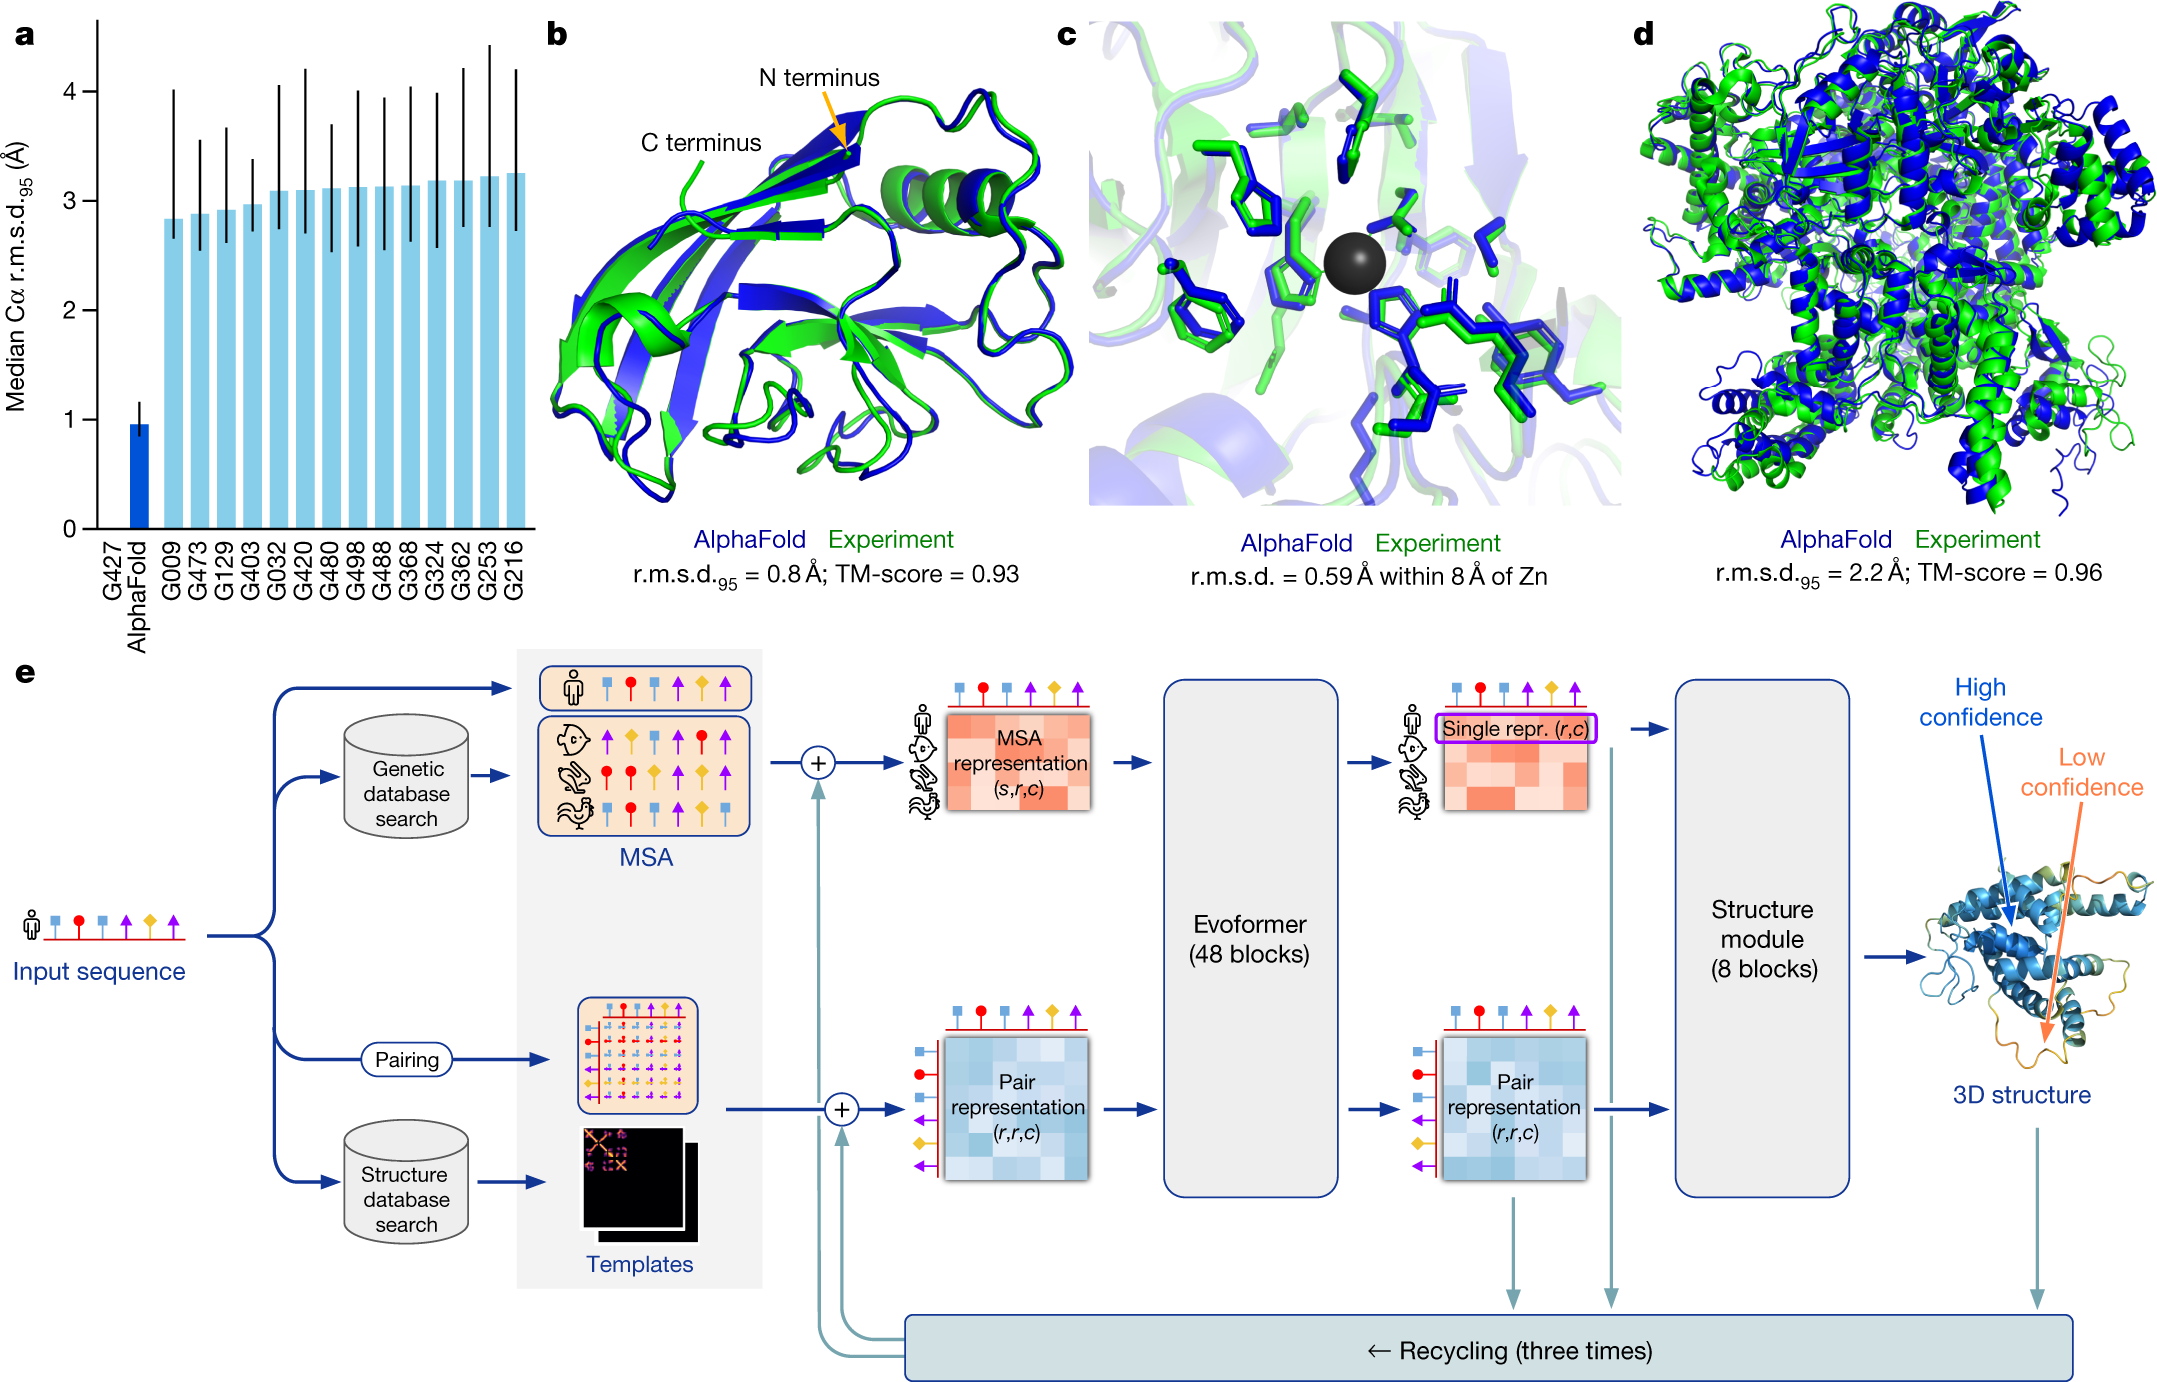
\includegraphics[width=.9\linewidth]{./img/AlphaFold_2.png}
\end{center}

J. Jumper \emph{et al}, 2020, Nature
(And \textgreater{} 50 years of data collection)
\end{frame}

\begin{frame}[label={sec:org937b50e}]{What are the DL techniques used in protein sequence generation?}
\begin{center}
\Large \textbf{Generative models to sample sequences}
\end{center}
\end{frame}
\begin{frame}[label={sec:orgc8aec73}]{Deep Generative Models}
\begin{itemize}
\item \alert{\alert{VAEs}}: Probabilistic; encoder-decoder structure.
\item \alert{\alert{GANs}}: Generator vs. discriminator competition.
\item \alert{\alert{RBMs}}: Energy-based with visible/hidden layers.
\item \alert{\alert{Normalizing Flows}}: Complex distribution transformations.
\item \alert{\alert{Autoregressive}}: Sequence prediction.
\item \alert{\alert{Energy-Based Models (EBMs)}}: Learn energy functions.
\end{itemize}

\begin{center}
\begin{center}
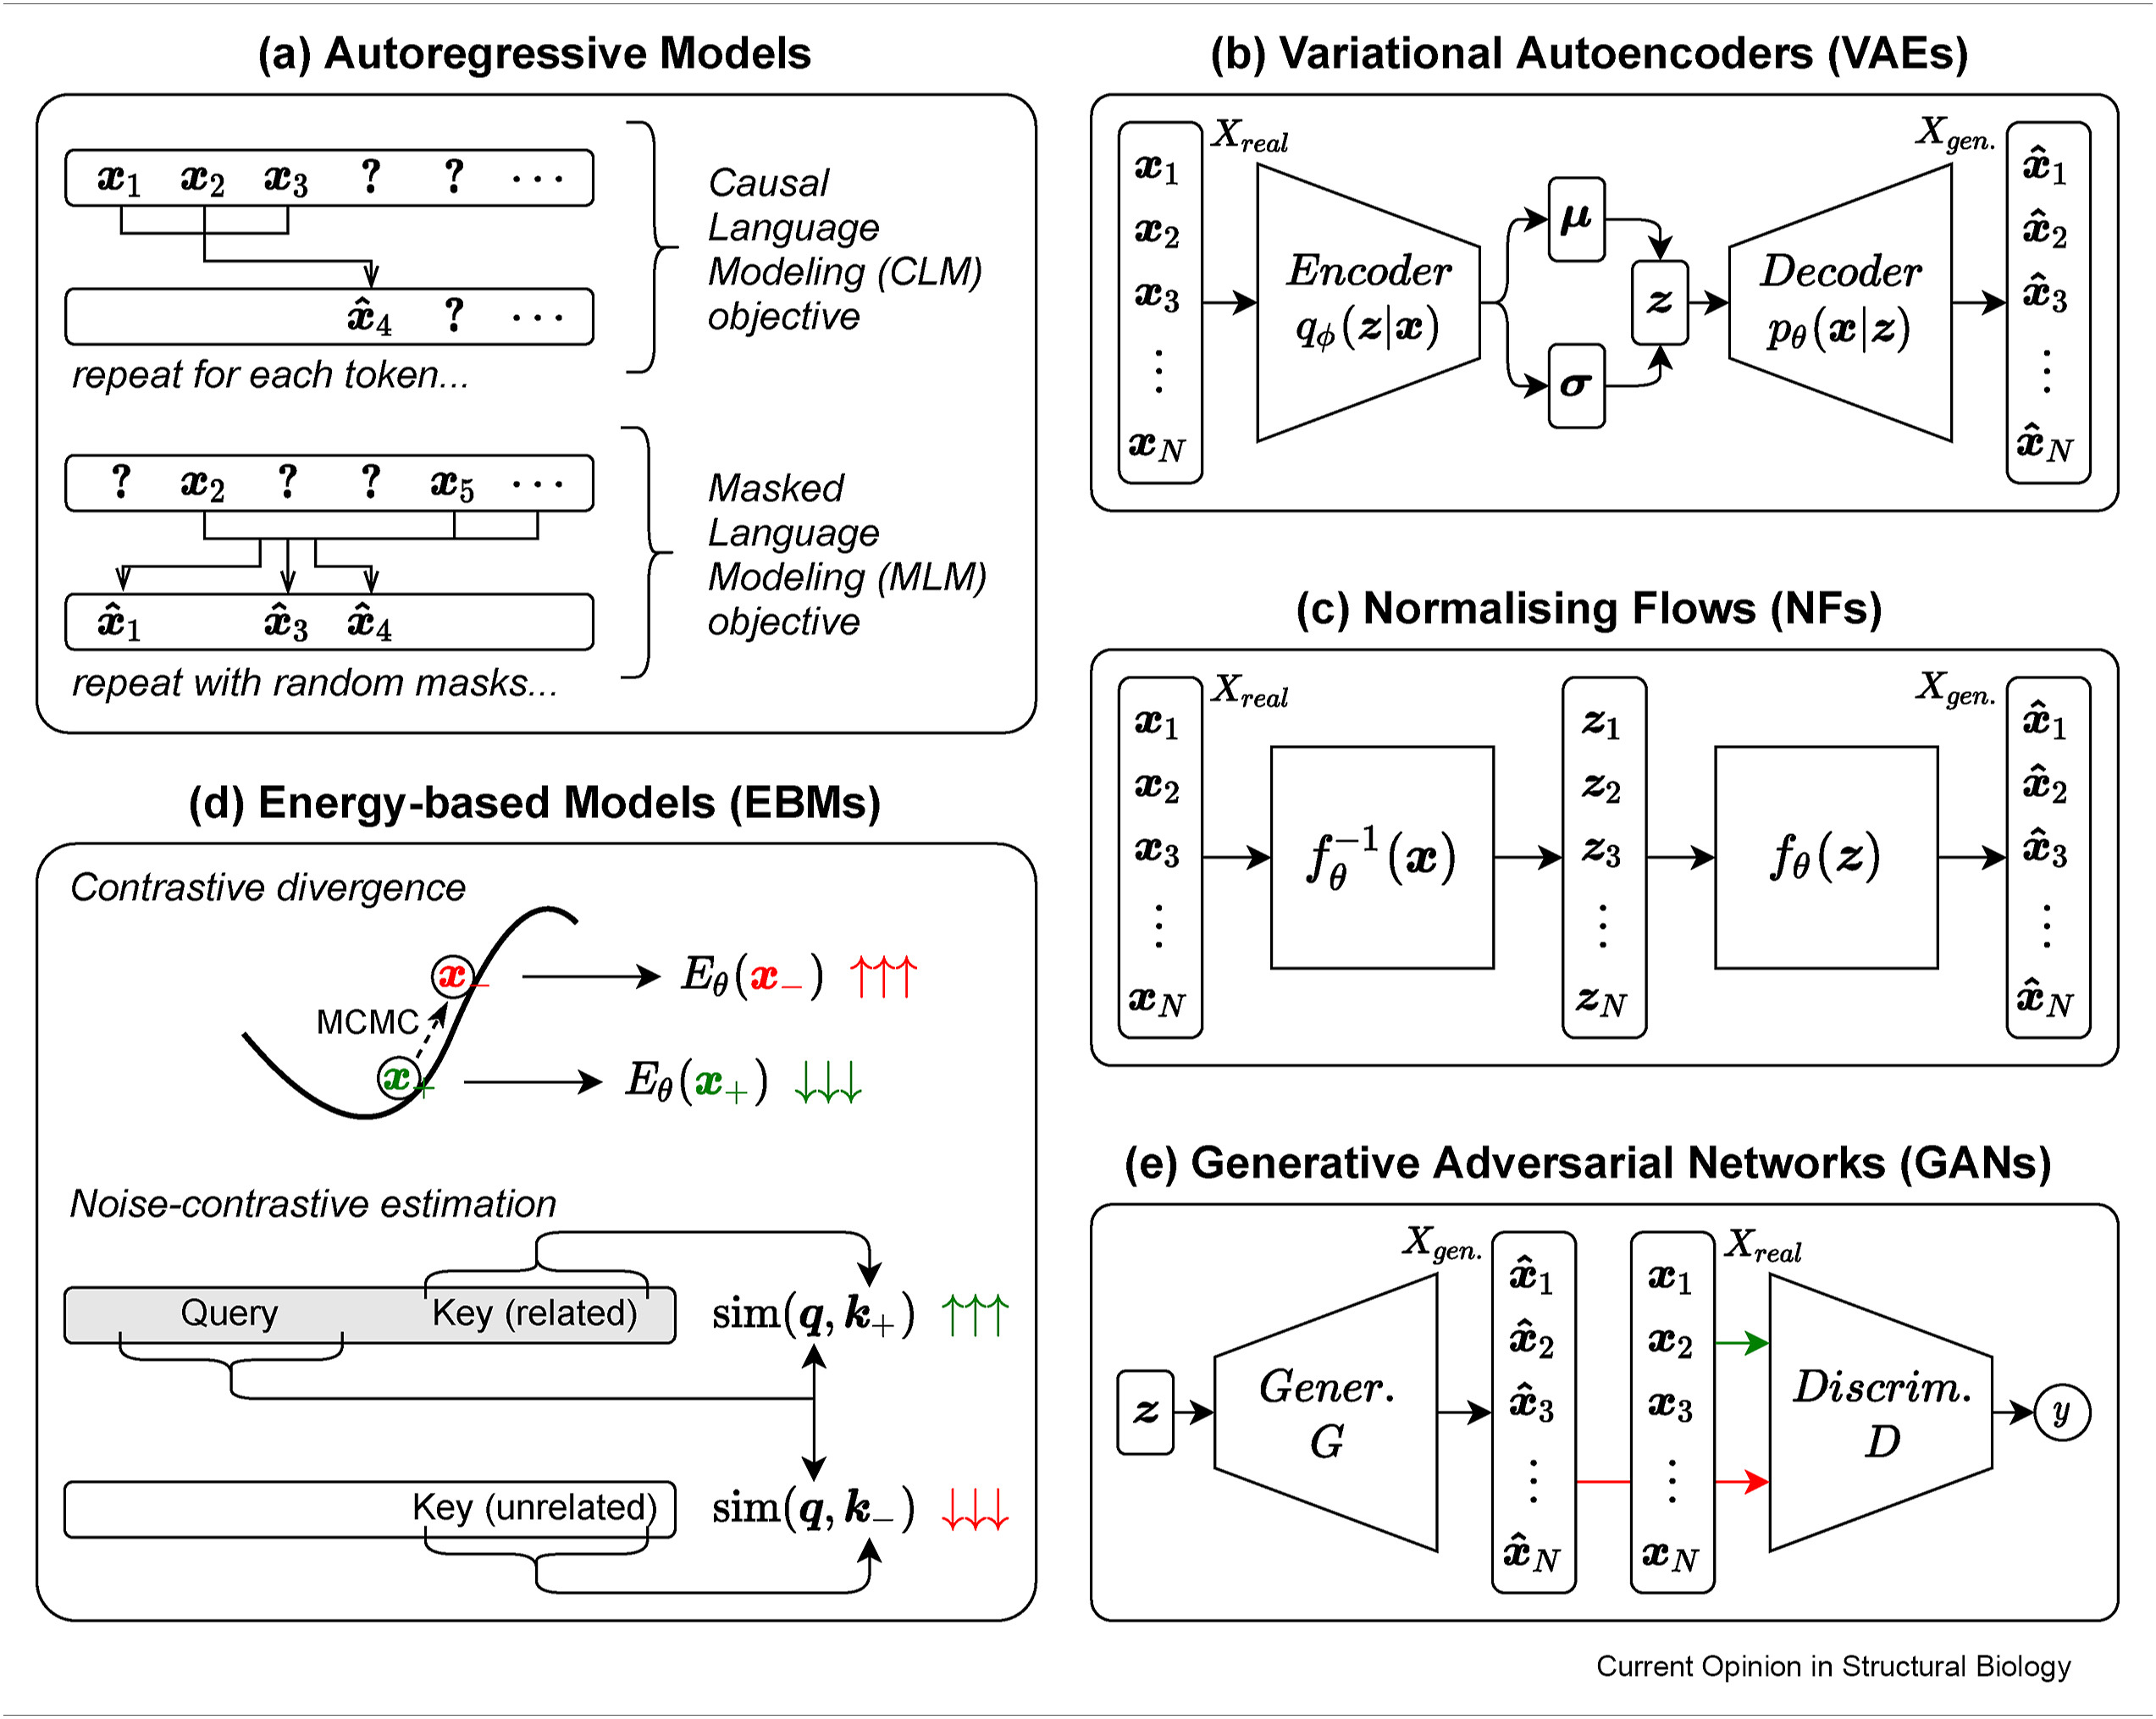
\includegraphics[scale=0.5]{./img/all_generative_models.jpg}
\end{center}
\end{center}
\end{frame}

\begin{frame}[label={sec:orgce52ea2}]{Variational Autoencoders (VAEs) in Protein Design}
\begin{columns}
\begin{column}{0.6\columnwidth}
\begin{itemize}
\item VAEs: Generative models that learn to encode and decode data.
\item Difference from standard autoencoders: Introduces probabilistic encoding.
\item Application: Generating functional protein sequences efficiently.
\end{itemize}
\end{column}

\begin{column}{0.4\columnwidth}
\begin{center}
\begin{center}
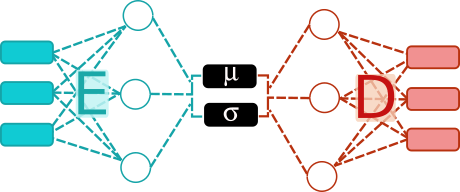
\includegraphics[width=.9\linewidth]{./img/VAE.png}
\end{center}
\end{center}
\end{column}
\end{columns}
\end{frame}

\begin{frame}[label={sec:org8bd5adb}]{Variational autoencoder framework [Ding \emph{et al}, 2020, Nat. Com.]}
\begin{center}
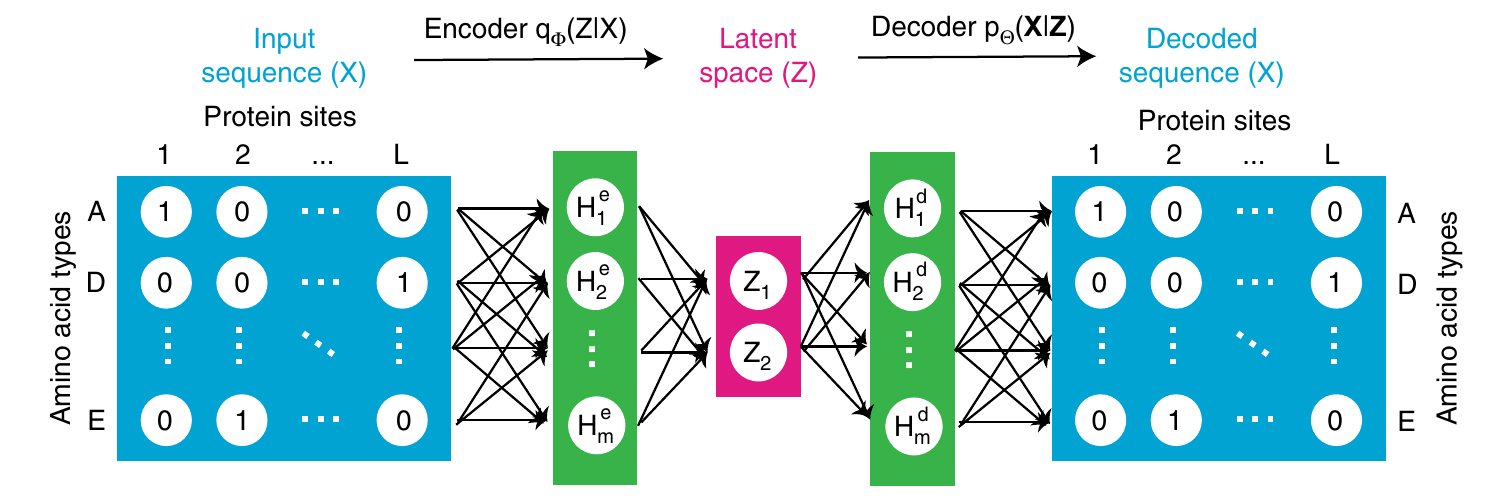
\includegraphics[width=.9\linewidth]{img/vae_scheme.png}
\end{center}
\begin{itemize}
\item Linear dense NN: \(H = W\times S + b\)
\item Activation function: \(ReLU(H_i) = max(0, H_i)\)
\item Output function: \(Softmax(X) = \hat{S} = \frac{exp\{X_i\}}{\sum\limits_{j}exp{X_j}}\)
\item \(Z \sim \mathcal{N}(\mu=0, \sigma^2=Id)\)
\end{itemize}
\begin{equation}
\begin{split}
  ELBO(\theta, \phi) &= \sum\limits_{Z} q_{\phi}(Z|X) \text{log} p_{\theta}(X|Z) - \sum\limits_{Z} q_{\phi}(Z|X) \text{log} \frac{q_{\phi}(Z|X)}{p_{\theta}(Z)}\\
  ELBO(\theta, \phi) &= <\mathcal{L}(\hat{S})> - D_{KL}(Encoder(S)||\mathcal{N}(Z|\mu, \sigma^2))
\end{split}
\end{equation}
\end{frame}

\begin{frame}[label={sec:org1b6ec9e}]{Training of a VAE}
\begin{block}{Architecture chosen by 5-fold cross validation}
\begin{itemize}
\item 1 \texttimes{} hidden (linear) layer fully connected (Encoder and Decoder)
\item 512 units per hidden layer
\item Latent space dimension = 10
\item Parameter space (W) dense layer: L \texttimes{} 21 \texttimes{} 512 \(\rightarrow\) 10\textsuperscript{6}
\end{itemize}
\end{block}
\begin{columns}
\begin{column}{0.5\columnwidth}
\begin{block}{Training paramerters}
\begin{itemize}
\item Re-weigting sequences (reduce redundancy and emphasize diversity)
\item 10\textsuperscript{4} optimization steps (ADAM optimizer)
\item Regularization
\end{itemize}
\end{block}
\end{column}

\begin{column}{0.5\columnwidth}
\begin{block}{Latent space representation of sequence space}
[Ding \emph{et al}, 2020, Nat. Com.]
\begin{center}
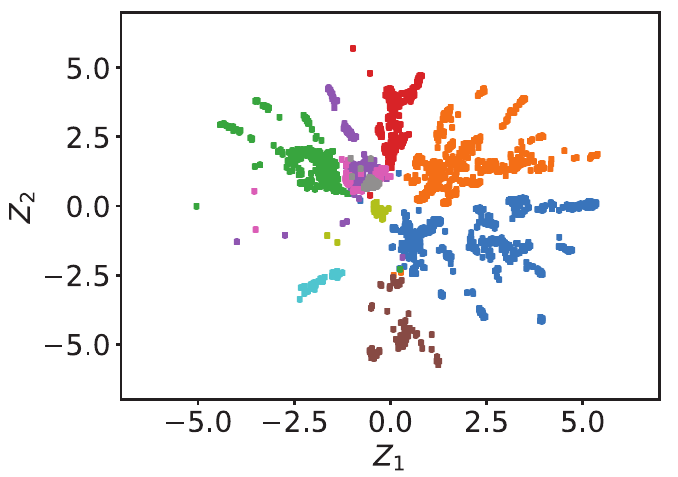
\includegraphics[width=.9\linewidth]{img/proj_prot_ding.png}
\end{center}
\end{block}
\end{column}
\end{columns}
\end{frame}

\begin{frame}[label={sec:org039d4e1}]{Use a structure predictor to deduce sequences}
\begin{center}
\Large \textbf{AlphaFold is so good at predicting the structure, can't we just invert it?}
Yes, we can!
\end{center}
\end{frame}

\begin{frame}[label={sec:org3b09c64}]{AlphaFold structure prediction}
\begin{center}
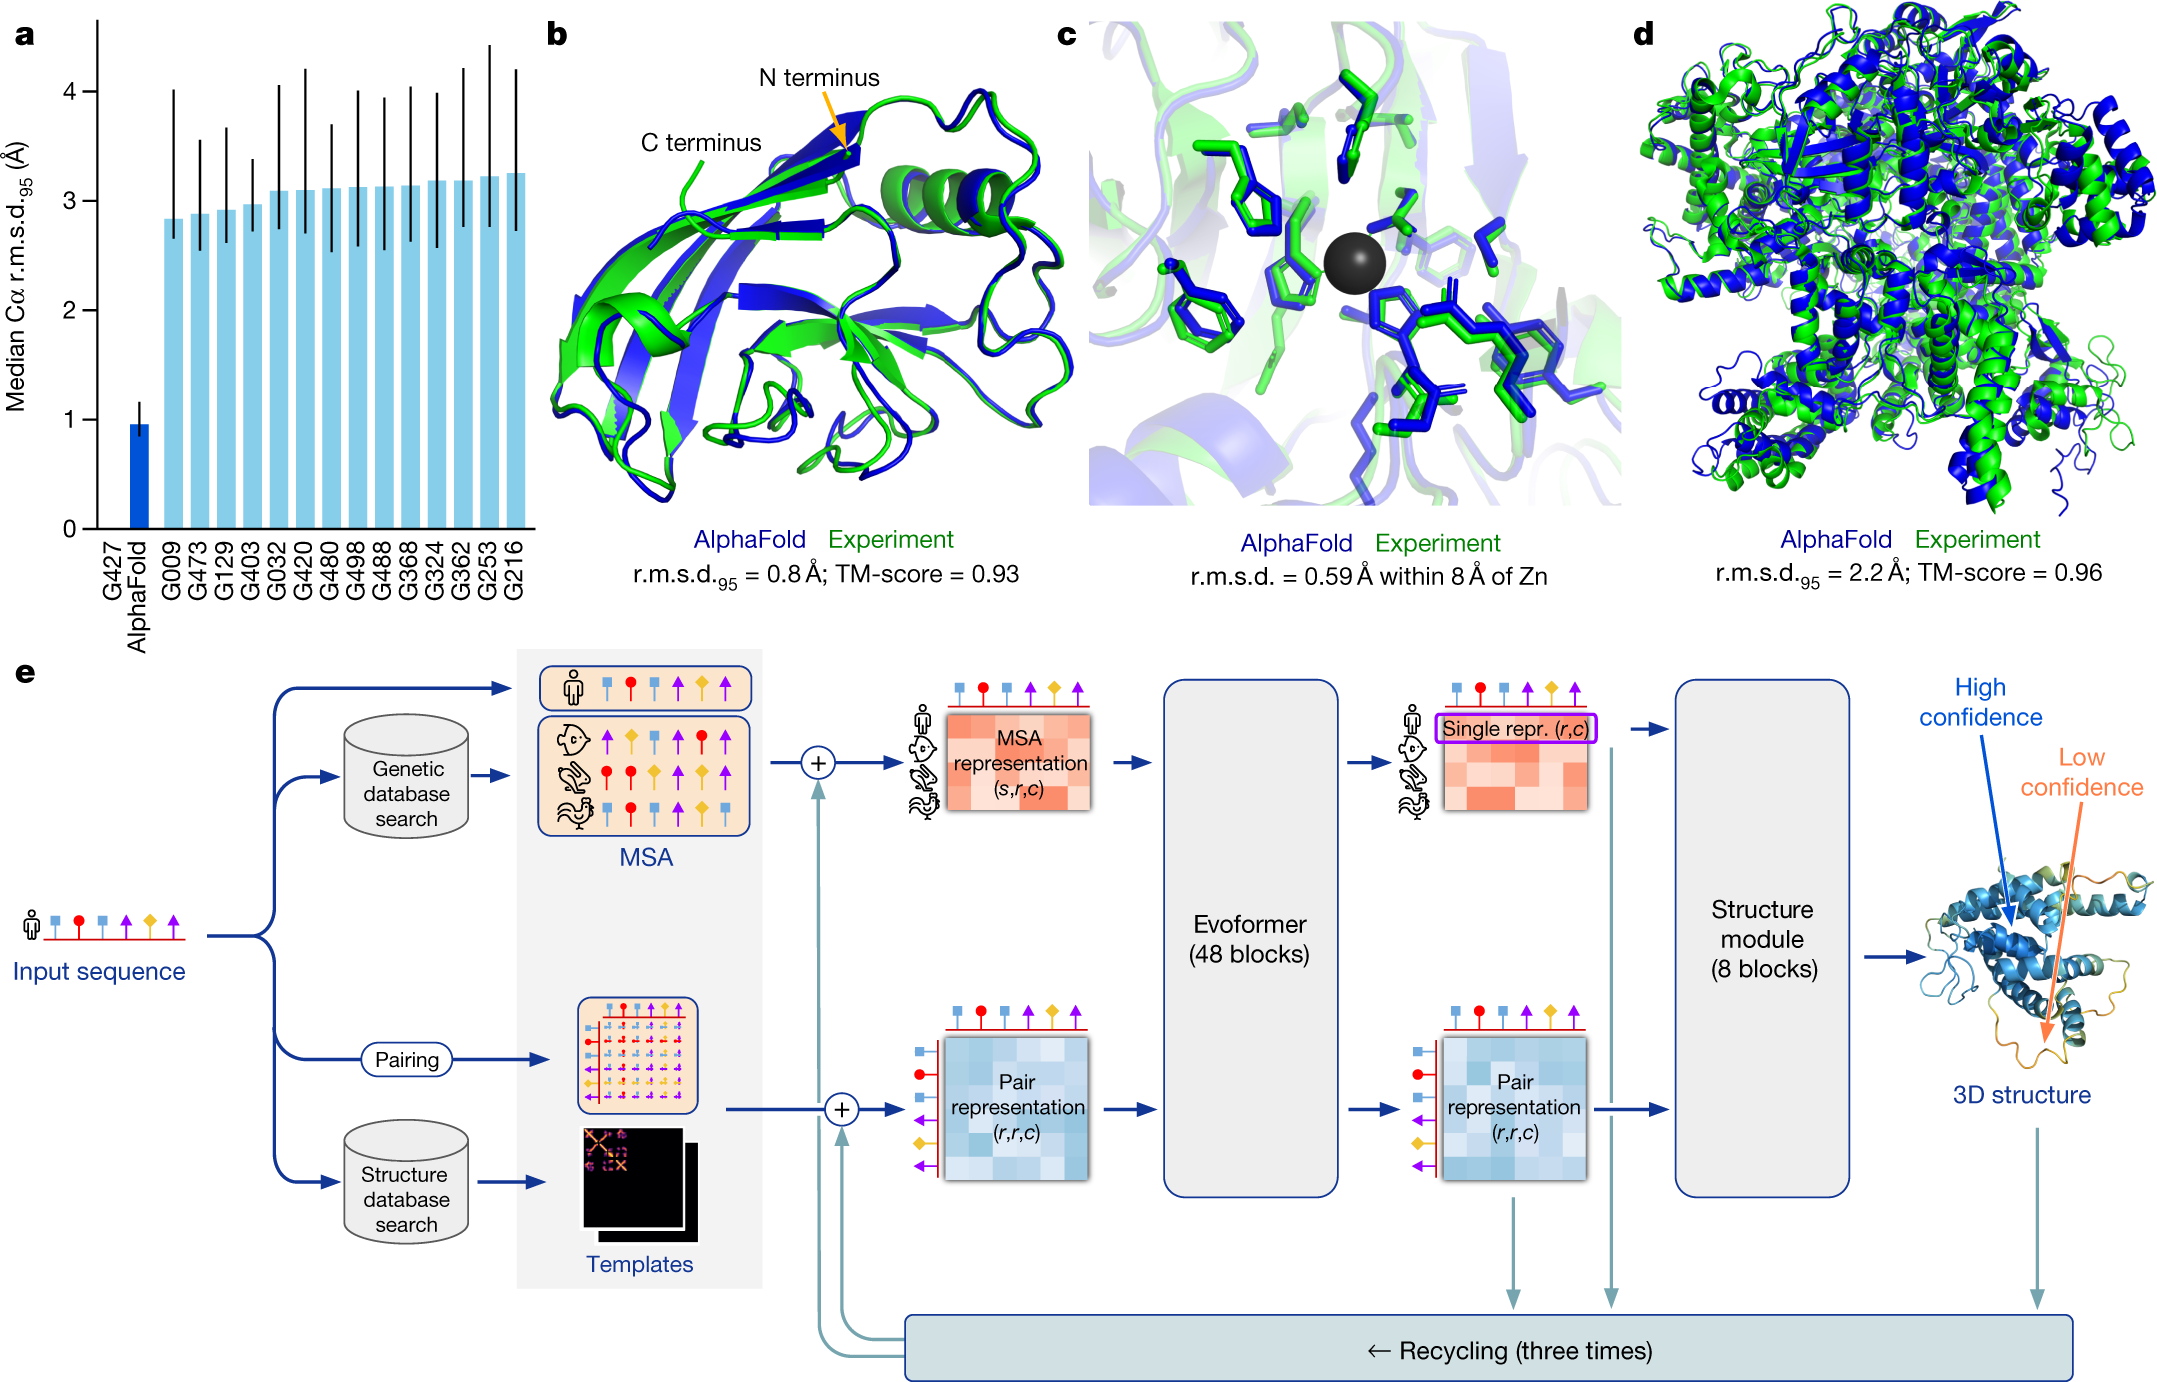
\includegraphics[width=.9\linewidth]{./img/AlphaFold_2.png}
\end{center}

End-to-End prediction model accounting for evolutionary information as well as
geometric information \(\rightarrow\) Any parameter on the way is differentiable,
even the input sequences.
\end{frame}

\begin{frame}[label={sec:orgfae0ef0}]{AlphaFold: inverting the prediction}
Prediction of a structure's fold.
\begin{center}
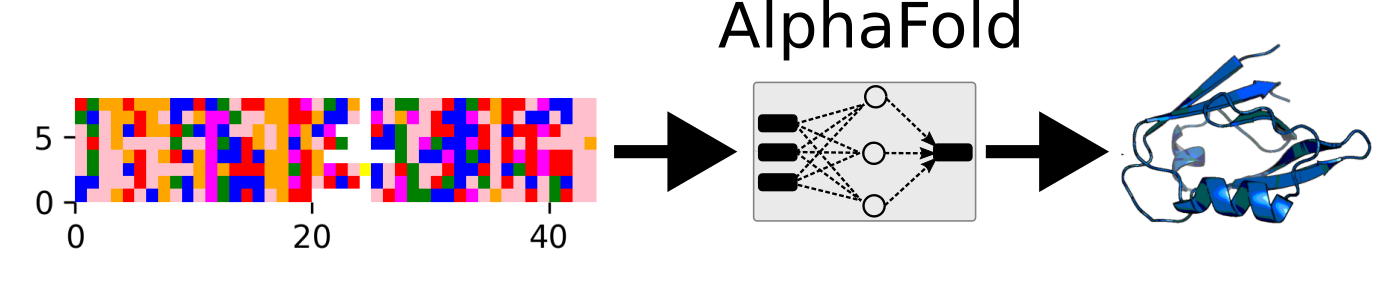
\includegraphics[width=.9\linewidth]{./img/af_1.png}
\end{center}

(J. Jumper \emph{et al}, 2020, Nature)
\end{frame}
\begin{frame}[label={sec:org5746914}]{AlphaFold: inverting the prediction}
Compare the prediction to the true structure and update accordingly the
parameters of AlphaFold using the \alert{gradient} of the loss function.

\begin{center}
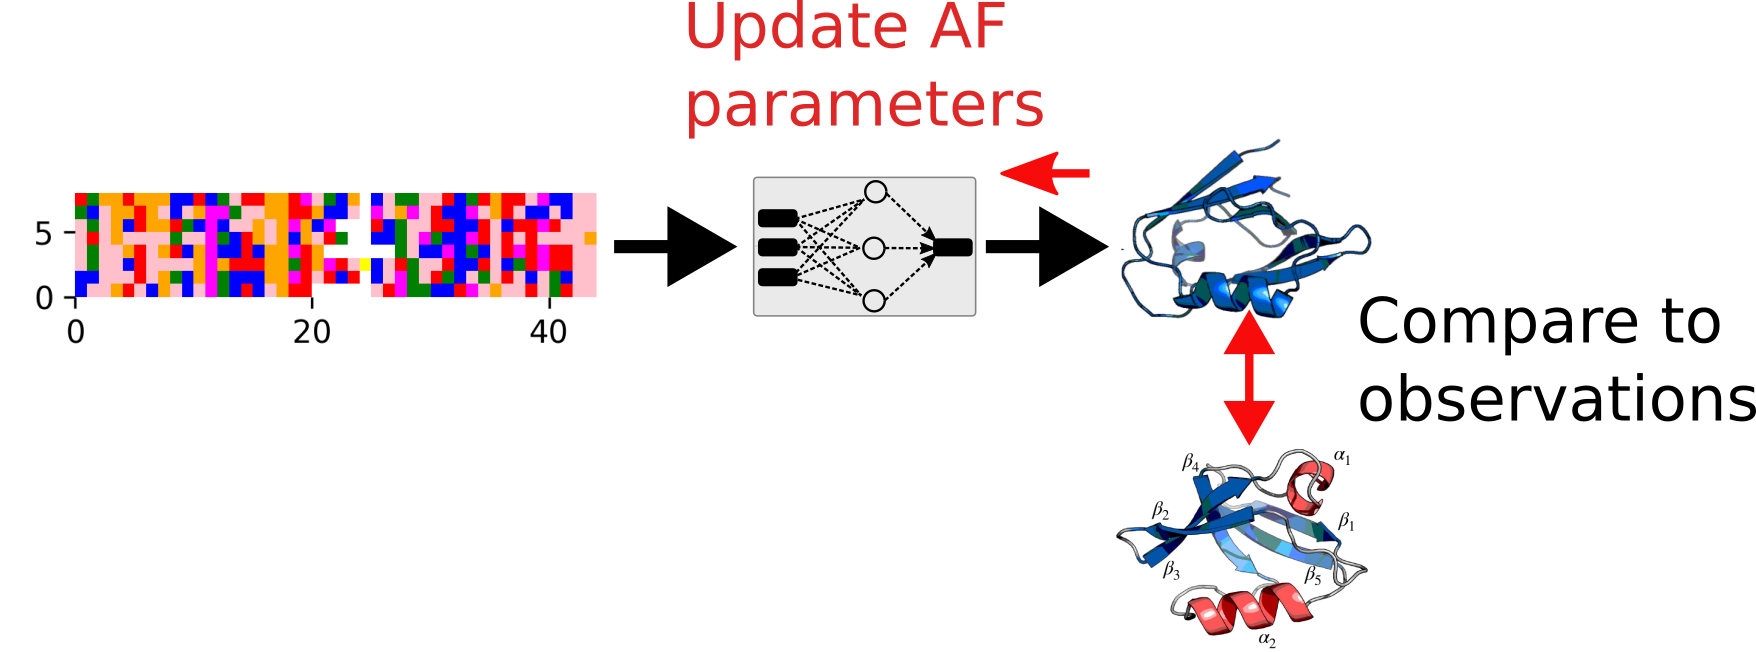
\includegraphics[width=.9\linewidth]{./img/af_2.png}
\end{center}
\end{frame}

\begin{frame}[label={sec:orgc15257d}]{AlphaFold: inverting the prediction}
\alert{\alert{To design}}: use the gradient with respect to the input only to search for
sequences that give the correct fold.

\begin{center}
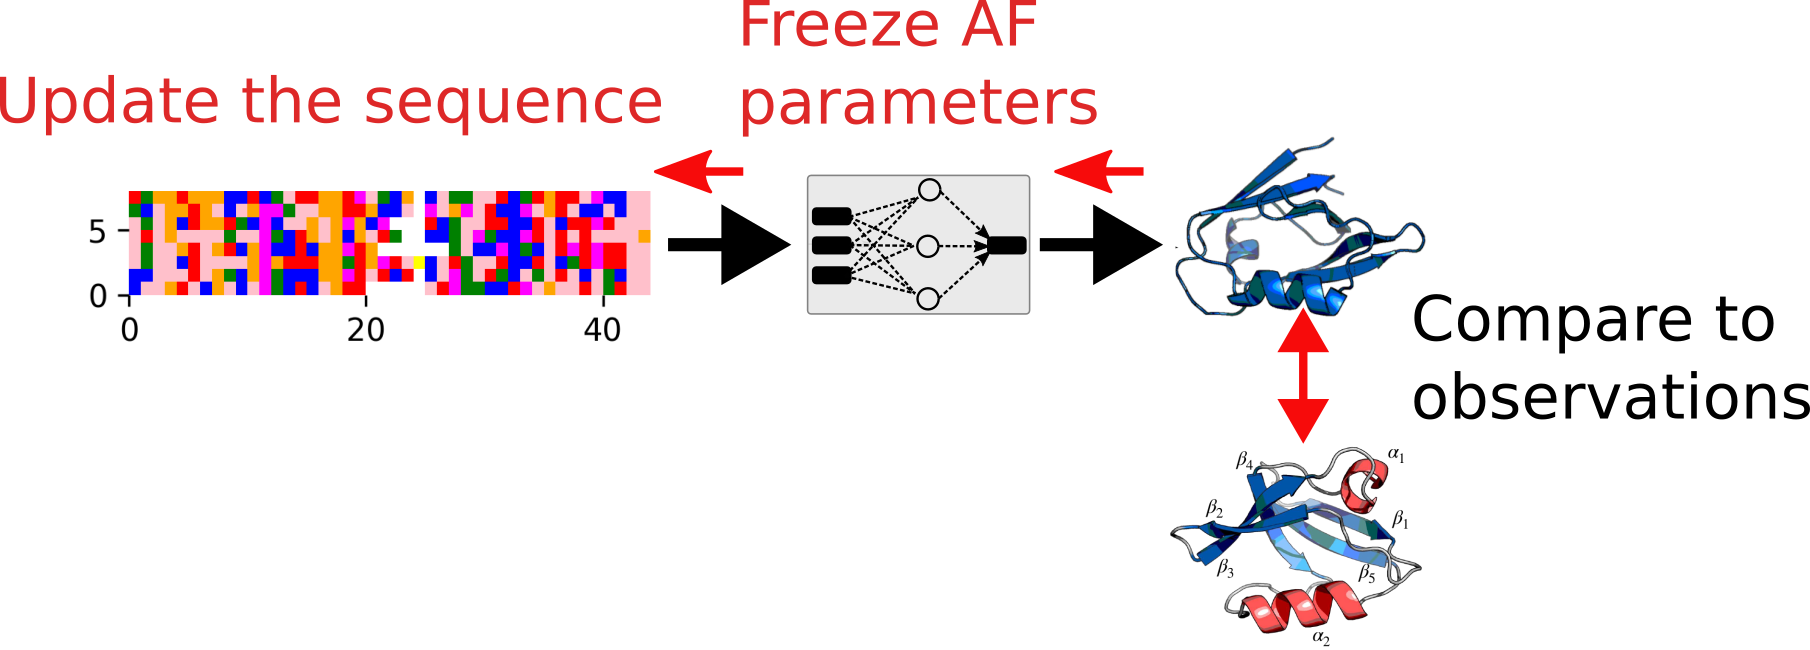
\includegraphics[width=.9\linewidth]{./img/af_3.png}
\end{center}
(Norm \emph{et al}, 2021, PNAS)
\end{frame}
\begin{frame}[label={sec:org84ac002}]{Reverting AlphaFold}
Encode the structure into distance matrices (D\textsubscript{i,j} = distance between residues
i and j).
\begin{center}
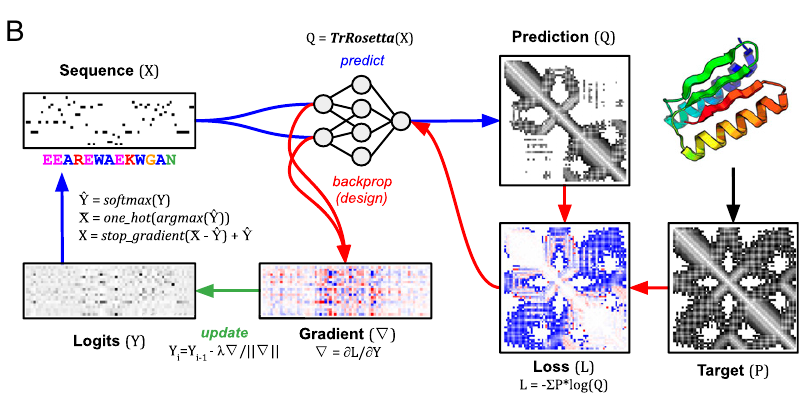
\includegraphics[width=.9\linewidth]{./img/af_optim_real.png}
\end{center}
(Norm \emph{et al}, 2021, PNAS)
\end{frame}
\begin{frame}[label={sec:orgc87f744}]{Why doing so?}
\begin{itemize}
\item Positive design: searching for sequences that fold into the target structure.
\item Negative design: searching for sequences that fold \alert{only} into the target structure.
\end{itemize}

\begin{center}
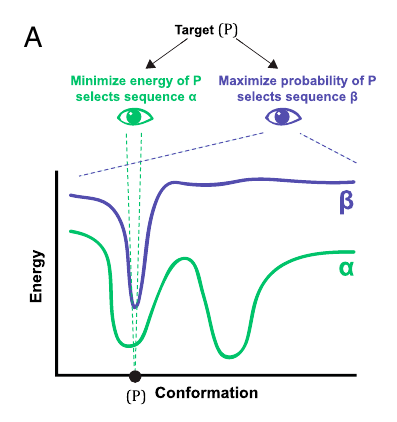
\includegraphics[scale=0.7]{./img/af_landscape_optimization.png}
\end{center}

(Norm \emph{et al}, 2021, PNAS)
\end{frame}

\begin{frame}[label={sec:org88e2d38}]{Graph neural network to model the structure}
\begin{center}
\Large \textbf{Represent protein structures using graph neural networks}
Yes, we can!
\end{center}
\end{frame}
\begin{frame}[label={sec:org5c42045}]{Design proteins conditioned on the structure}
\begin{center}
\includegraphics[width=.9\linewidth]{./img/proteinmpnn.jpg}
\end{center}
[Dauparas \emph{et al}, Science, 2022]
\end{frame}

\begin{frame}[label={sec:org59a5771}]{Graph neural network}
\begin{columns}
\begin{column}{0.5\columnwidth}
\begin{center}
\includegraphics[width=.9\linewidth]{img/p1.png}
\end{center}
\end{column}

\begin{column}{0.5\columnwidth}
\begin{center}
\includegraphics[width=.9\linewidth]{img/mol_graph.png}
\end{center}
[Gilmer \emph{et al}, ICML, 2017]
\end{column}
\end{columns}
\end{frame}

\begin{frame}[label={sec:orgb6b451d}]{Graph neural network}
\begin{columns}
\begin{column}{0.5\columnwidth}
\begin{center}
\includegraphics[width=.9\linewidth]{img/p2.png}
\end{center}
\end{column}

\begin{column}{0.5\columnwidth}
\begin{center}
\includegraphics[width=.9\linewidth]{img/mol_graph.png}
\end{center}
[Gilmer \emph{et al}, ICML, 2017]
\end{column}
\end{columns}
\end{frame}
\begin{frame}[label={sec:org31a7a4a}]{Graph neural network}
\begin{columns}
\begin{column}{0.5\columnwidth}
\begin{center}
\includegraphics[width=.9\linewidth]{img/p3.png}
\end{center}
\end{column}

\begin{column}{0.5\columnwidth}
\begin{center}
\includegraphics[width=.9\linewidth]{img/mol_graph.png}
\end{center}
[Gilmer \emph{et al}, ICML, 2017]
\end{column}
\end{columns}
\end{frame}
\begin{frame}[label={sec:org80836fa}]{Graph neural network}
\begin{columns}
\begin{column}{0.5\columnwidth}
\begin{center}
\includegraphics[width=.9\linewidth]{img/p4.png}
\end{center}
\end{column}

\begin{column}{0.5\columnwidth}
\begin{center}
\includegraphics[width=.9\linewidth]{img/mol_graph.png}
\end{center}
[Gilmer \emph{et al}, ICML, 2017]
\end{column}
\end{columns}
\end{frame}
\begin{frame}[label={sec:org0c00959}]{Graph neural network}
\begin{columns}
\begin{column}{0.5\columnwidth}
\begin{center}
\includegraphics[width=.9\linewidth]{img/p5.png}
\end{center}
\end{column}

\begin{column}{0.5\columnwidth}
\begin{center}
\includegraphics[width=.9\linewidth]{img/mol_graph.png}
\end{center}
[Gilmer \emph{et al}, ICML, 2017]
\end{column}
\end{columns}
\end{frame}
\begin{frame}[label={sec:org88c2622}]{Graph neural network}
\begin{columns}
\begin{column}{0.5\columnwidth}
\begin{center}
\includegraphics[width=.9\linewidth]{img/p6.png}
\end{center}
\end{column}

\begin{column}{0.5\columnwidth}
\begin{center}
\includegraphics[width=.9\linewidth]{img/mol_graph.png}
\end{center}
[Gilmer \emph{et al}, ICML, 2017]
\end{column}
\end{columns}
\end{frame}
\begin{frame}[label={sec:org3afd185}]{Graph neural network}
\begin{columns}
\begin{column}{1\columnwidth}
\begin{center}
\includegraphics[width=.9\linewidth]{img/p7.png}
\end{center}

Predict a molecular property using the contextualized node vectors, for example,
the binding free energy to a protein target.
\end{column}
\end{columns}
\end{frame}

\begin{frame}[label={sec:orgd1f49bd}]{Graph neural network}
\begin{columns}
\begin{column}{0.5\columnwidth}
\begin{center}
\includegraphics[width=.9\linewidth]{img/p8.png}
\end{center}

Mask the identity of one atom\ldots{}
\end{column}

\begin{column}{0.5\columnwidth}
\begin{center}
\includegraphics[width=.9\linewidth]{img/mol_graph.png}
\end{center}
[Gilmer \emph{et al}, ICML, 2017]
\end{column}
\end{columns}
\end{frame}
\begin{frame}[label={sec:orga22fad1}]{Graph neural network}
\begin{columns}
\begin{column}{0.5\columnwidth}
\begin{center}
\includegraphics[width=.9\linewidth]{img/p9.png}
\end{center}

\ldots{}predict back the identity of the masked atom.
\end{column}

\begin{column}{0.5\columnwidth}
\begin{center}
\includegraphics[width=.9\linewidth]{img/mol_graph.png}
\end{center}
[Gilmer \emph{et al}, ICML, 2017]
\end{column}
\end{columns}
\end{frame}
\end{document}